\section{Problème}

Données deux interfaces (1 et 2) séparant respectivement les milieux 1 et 2 (de paramètres $\rho_1,c_1$ et $\rho_2,c_2$)
et les milieux 2 et 1.

Une onde acoustique vient frapper la première interface en un point $A$ avec un angle à la normale $\theta_1$. L'onde
transmise dans le milieu 2 vient rencontrer ensuite une seconde interface où une partie est transmise à nouveau vers le
milieu 1 (voir figure~\ref{complete}). On se propose de calculer et de tracer les coefficients de réflexion $R$ et
transmission $T$ du problème (on utilisera, au besoin les coefficients $R_i$ et $T_i$ à chacune des deux interfaces
--- $i\in\{1;2\}$).

\subsection{Conditions du problème}

Nous étudierons d'abord la première interface puis la seconde. Les conditions suivantes sont supposées à
chacune des deux interfaces :

\begin{itemize}
    \item Condition de Sommerfeld : on ne considère pas d'onde retour
    \item Condition à l'interface : continuité de la pression et de la vitesse normale à l'interface.
\end{itemize}

De plus, les ondes seront considérées monochromatiques.

\subsection{Notations}

Les pressions incidente, réfléchie et transmise à l'interface $i$ seront notées $\pI_i$, $\pR_i$ et $\pT_i$, les
vitesses normales aux deux interfaces, elles, seront notées : $\vI_i$, $\vR_i$ et $\vT_i$.

\subsection{Schéma du problème}

Le problème peut être schématisé comme montré en figure~\ref{complete}.

\begin{figure}[!b]
    \centering{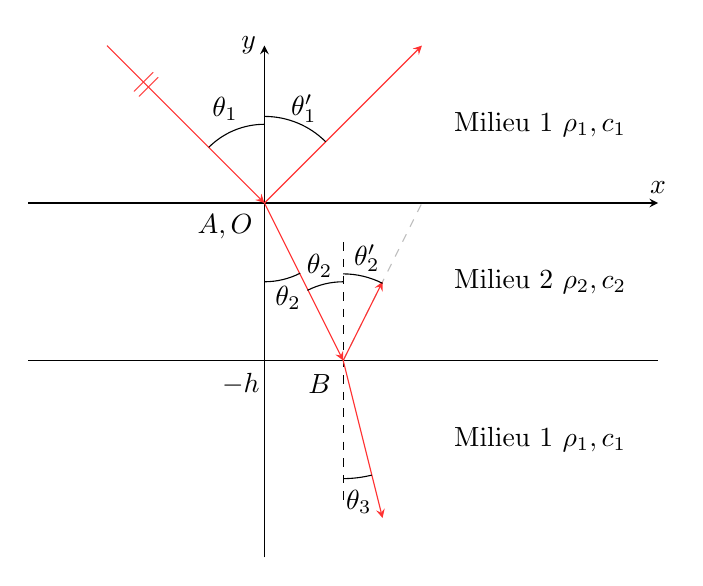
\begin{tikzpicture}

    % ifaces
    \draw [>=stealth, ->] (-3,0) -- (5,0);
    \draw (-3,-2) -- (5,-2);

    % Labels
    \draw (3.5,1) node {Milieu 1 $\rho_1,c_1$};
    \draw (3.5,-1) node {Milieu 2 $\rho_2,c_2$};
    \draw (3.5,-3) node {Milieu 1 $\rho_1,c_1$};

    % verticals
    \draw [dashed] (0,1.5) -- (0,-1.5);
    \draw [dashed] (1,-0.5) -- (1,-3.8);

    % axis
    %% y
    \draw [>=stealth, ->] (0,-4.5) -- (0,2);
    \draw (-.2,2) node {$y$};
    %% x (already drawn)
    \draw (5,.2) node {$x$};
    %% ordonnée h
    \draw (-.3,-2.3) node {$-h$};


    % points A & B
    \draw (-.5, -.3) node {$A,O$};
    \draw (.7, -2.3) node {$B$};

    % rays
    \draw [red!80, >=stealth, ->] (-2,2) -- (0,0) node[near start, sloped] {$| |$};
    \draw [red!80, >=stealth, ->] (0,0) -- (2,2);
    \draw [red!80, >=stealth, ->] (0,0) -- (1, -2);
    \draw [gray!50, dashed] (1,-2) -- (2,0);
    \draw [red!80, >=stealth, ->] (1,-2) -- (1.5, -1);
    \draw [red!80, >=stealth, ->] (1,-2) -- (1.5, -4);

    % angles
    \draw (0,1) arc (90:135:1) node at (-0.5,1.2) {$\theta_1$};
    \draw (0,1.1) arc (90:45:1.1) node at (0.5,1.2) {$\theta_1'$};
    \draw (0,-1) arc (-90:-63:1) node at (0.3,-1.2) {$\theta_2$};
    \draw (1,-1) arc (90:117:1) node at (.7,-.8) {$\theta_2$};
    \draw (1,-0.9) arc (90:63:1.1) node at (1.3,-.7) {$\theta_2'$};
    \draw (1,-3.5) arc (-90:-76:1.5) node at (1.2,-3.8) {$\theta_3$};


\end{tikzpicture}

}
    \caption{\label{complete} Schématisation complète du problème}
\end{figure}

